%-----appendices
\begin{appendices}
\noappendicestocpagenum
\addappheadtotoc
\chapter{Checklist for cooldown}
%-----appendices
\label{appendix:checklist-for-cooldown}

\begin{figure}[!htbp]
 \centering
 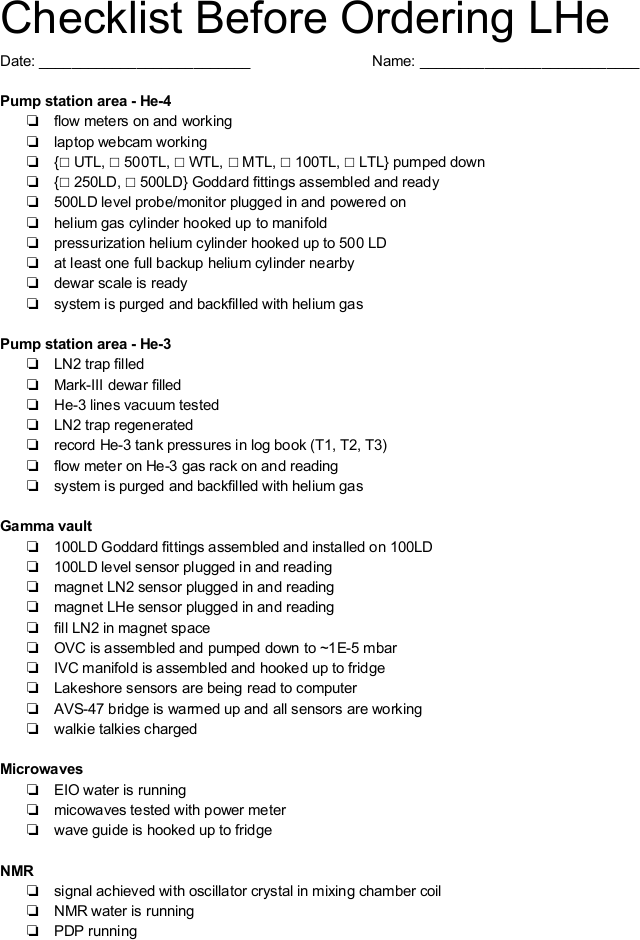
\includegraphics[height=.95\textheight]{./docs/cooldown-checklist.png}
 % cooldown-checklist.pdf: 0x0 pixel, 0dpi, 0.00x0.00 cm, bb=
 \caption{Checklist.}
 \label{fig:checklist}
\end{figure}



\chapter{SLPM Conversion}
\label{appendix:slpm-conversion}
Some HiFrost documents from CERN refer to flow rates of \hef{} and \het{} in millimoles per second.  The formula to convert this flow rate to SLPM is
\begin{equation}
 \textrm{[SLPM]}=\left(\frac{60\textrm{ s}}{\textrm{min}}\right)\left(\frac{x\textrm{ mol}}{\textrm{s}}\right)\left(\frac{4\textrm{ g}}{\textrm{mol}}\right)\left(\frac{1\textrm{ L}}{0.1785\textrm{ g}}\right)
\end{equation}
for \hef{} and 

\begin{equation}
 \textrm{[SLPM]}=\left(\frac{60\textrm{ s}}{\textrm{min}}\right)\left(\frac{x\textrm{ mol}}{\textrm{s}}\right)\left(\frac{3.01\textrm{ g}}{\textrm{mol}}\right)\left(\frac{1\textrm{ L}}{0.135\textrm{ g}}\right)
\end{equation}
for \het{}\cite{linde-helium-3-sheet}, where [SLPM] is the standard flow volume, $x$ is the flow rate in mol/s, $k$ is the Boltzmann constant and the definitions for STP are a temperature of 273.15 K and a pressure of 100 kPa.

Figure \ref{fig:slpm-conversion} shows some values of SLPM to mmol/s flow.

\begin{figure}
\begin{tabular}{|c|c|c|}
\hline
 SLPM& mmol/s (\het)& mmol/s (\hef)\\
\hline
5&3.74&3.71\\
\hline
10&7.48&7.44\\
\hline
15&11.21&11.16\\
\hline
20&14.95&14.86\\
\hline
25&18.69&18.60\\
\hline
30&22.42&22.31\\
\hline
40&29.90&29.75\\
\hline
50&37.38&37.19\\
\hline
60&44.85&44.63\\
\hline
80&59.80&59.50\\
\hline
100&74.75&74.38\\
\hline

\end{tabular}
\caption{Flow rate conversion between mmol/s to SLPM for helium.}
\label{fig:slpm-conversion}
\end{figure} 
\end{appendices}